
\thispagestyle{empty}

\vspace*{-\headsep}
\noindent%
\begin{minipage}[c][\textheight][c]{\linewidth}

\noindent%
\begin{minipage}{\linewidth}
\raggedright

\section{Your Real Home}

Your external home is not your real home. It is your\linebreak\ supposed home, your home in the world. As for your real home, that's peace. The Buddha has us build our own home by letting go till we reach peace.

\end{minipage}

\end{minipage}

\AddToShipoutPicture*{\put(\LenToUnit{3in},\LenToUnit{2.5in}){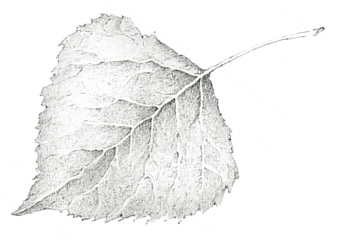
\includegraphics[width=0.6in,keepaspectratio,angle=190]{birch_by_Aj_Vimalo_3_CMYK.png}}}

\clearpage

\section{To the Ocean}

The streams, lakes, and rivers that flow down to the ocean, when they reach the ocean, all have the same blue color, the same salty taste.

The same with human beings: it doesn't matter where they're from -- when they reach the stream of the Dhamma, it's all the same Dhamma.

\section{Groundwater}

The Buddha is the Dhamma; the Dhamma is the Buddha. The Dhamma the Buddha awakened to is something always there in the world. It hasn't disappeared. It's like groundwater. Whoever digs a well down to the level of the groundwater will see water. It's not the case that that person created or fashioned the water into being. All he's done is to put his strength into digging the well so that it's deep enough to reach the water already there.

So if we have any discernment, we'll realize that we're not far from the Buddha at all. We're sitting right in front of him right now. Whenever we understand the Dhamma, we see the Buddha. Those who are intent on practicing the Dhamma continuously -- wherever they sit, stand, or walk -- are sure to hear the Buddha's Dhamma at all times.

\clearpage

\section{It's All Right Here}

The Buddha is the Dhamma; the Dhamma is the Buddha. He didn't take away the knowledge he awakened to. He left it right here. To put it in simple terms, it's like the teachers in schools. They haven't been teachers from birth. They had to study the course of study for teachers before they could be teachers, teaching in school and getting paid. After a while, they'll die away -- away from being teachers. But you can say that in a way the teachers don't die. The qualities that make people into teachers remain right here. It's the same with the Buddha. The noble truths that made him the Buddha still remain right here. They haven't run off anywhere at all.

\section{The Roots}

We're like a tree with roots, a base, and a trunk. Every leaf, every branch, depends on the roots to absorb nutrients from the soil and send them up to nourish the tree.

Our body, plus our words and deeds, our senses of sight, hearing, smell, taste, and feeling, are like the branches, leaves, and trunk. The mind is like the roots absorbing nutrients and sending them up the trunk to the leaves and branches so that they flower and bear fruit.

\clearpage

\section{Elephants, Oxen, and Water Buffaloes}

Training the mind well is a useful activity. You can see this even in draft animals, like elephants, oxen, and water buffaloes. Before we can put them to work, we have to train them. Only when they're well trained can we use their strength and put it to different purposes. All of you know this. 

A mind well trained is of many times greater value. Look at the Buddha and his noble disciples. They changed their status from being run-of-the-mill people to being noble ones, respected by people all over. And they've benefited us in more wide-ranging ways than we could ever determine. All of this comes from the fact that they've trained their minds well.

A mind well trained is of use in every occupation. It enables us to do our work with circumspection. It makes us reasonable instead of impulsive, and enables us to experience a happiness appropriate to our station in life.

\clearpage

\section{The Lost Wallet}

It's as if you leave home and lose your wallet. It fell out of your pocket onto the road away back there, but as long as you don't realize what happened you're at ease -- at ease because you don't yet know what this ease is for. It's for the sake of dis-ease at a later time. When you eventually see that you've really lost your money: that's when you feel dis-ease -- when it's right in your face. 

The same holds true with our bad and good actions. The Buddha taught us to acquaint ourselves with these things. If we aren't acquainted with these things, we'll have no sense of right or wrong, good or bad.

\section{Leaves}

When we sit in a quiet forest when there's no wind, the leaves are still. When the wind blows, the leaves flutter.

The mind is the same sort of thing as leaves. When it makes contact with an object, it vibrates in line with its nature. The less you know of the Dhamma, the more the mind vibrates. When it feels pleasure, it dies with the pleasure. When it feels pain, it dies with the pain. It keeps flowing on in this way. 

\clearpage

\section{A Block of Ice}

If you place a large block of ice out in the open sun, you can see it deteriorate -- in the same way the body ages -- bit by bit, bit by bit. After only a few minutes, only a few hours, it will all melt into water. This is called \textit{khaya-vaya:} ending, deterioration.

The deterioration of fabricated things has been going on for a long time, ever since the world came into being. When we're born, we take on these things as well. We don't discard them anywhere. When we're born, we take on illness, aging, and death. We gather them up at the same time.

Look at the ways it deteriorates, this body of ours. Every part deteriorates. Hair of the head deteriorates; hair of the body deteriorates; fingernails and toenails deteriorate; skin deteriorates. Everything, no matter what, deteriorates in line with its nature.

\clearpage

\section{Wagon Wheels, Wagon Tracks}

The cycle of rebirth is like a wagon wheel. An ox is pulling the wagon. If it keeps on pulling the wagon without stopping, the wagon tracks will keep on erasing the ox tracks without stop. The wagon wheels aren't long, but they're round. You could say that they're long, but their length is round. We see their roundness but we don't see their length. As long as the ox pulls without stopping, the wagon wheels turn without stopping. 

On a later day the ox stops. It's tired. It drops the yoke. The ox then goes its way, the wagon goes its way. The wagon wheels stop of their own accord. If you leave them there a long time, they disintegrate into earth, water, wind, and fire, turning back into grass and dirt.

It's the same with people who are still making kamma: they don't come to closure. People speaking the truth don't come to closure. People with wrong views don't come to closure.

\clearpage

\section{Children, Bullets}

A gun shoots its children -- its bullets -- outward. We shoot ours inward, into our heart. When they're good, we're shot in the heart. When they're bad, we're shot in the heart. They're an affair of kamma, our children. There are good ones, there are bad ones, but both the good and bad are our children all the same. 

When they're born, look at us: the worse off they are, the more we love them. If one of them comes down with polio and gets crippled, that's the one we love the most. When we leave the house we tell the older ones, `Look after your little sister. Look after this one' -- because we love her. When we're about to die we tell them, `Look after her. Look after my child.' She's not strong, so you love her even more.

\clearpage

\section{The Tail of the Snake}

\enlargethispage{\baselineskip}
We human beings don't want suffering. We want nothing but pleasure. But actually, pleasure is nothing but subtle suffering. Pain is blatant suffering. To put it in simple terms, suffering and pleasure are like a snake. Its head is suffering; its tail is pleasure. Its head contains poison. Its mouth contains poison. If you get near its head, it'll bite you. If you catch hold of its tail it seems safe, but if you hold onto its tail without letting go, it can turn around and bite you just the same. That's because both the head of the snake and the tail of the snake are on the same snake.

Both happiness and sadness come from the same parents: craving and delusion. That's why there are times when you're happy but still restless and ill at ease -- even when you've got things you like, such as material gain, status, and praise. When you get these things you're happy, but your mind isn't really at peace because there's still the sneaking suspicion that you'll lose them. You're afraid they'll disappear. This fear is the cause that keeps you from being at peace. Sometimes you actually do lose these things and then you really suffer. This means that even though these things are pleasant, suffering lies fermenting in the pleasure. We're simply not aware of it. Just as when we catch hold of a snake: even though we catch hold of its tail, if we keep holding on without letting go, it can turn around and bite us.

So the head of the snake and the tail of the snake, evil and goodness: these form a circle that keeps turning around. That's why pleasure and pain, good and bad are not the path.

\clearpage

\section{The King of Death}

We live like a chicken who doesn't know what's going on. In the morning it takes its baby chicks out to scratch for food. In the evening, it goes back to sleep in the coop. The next morning it goes out to look for food again. Its owner scatters rice for it to eat every day, but it doesn't know why its owner is feeding it. The chicken and its owner are thinking in very different ways.

The owner thinks, `How much does the chicken weigh?' The chicken, though, is engrossed in the food. When the owner picks it up to feel its weight, it thinks the owner is showing affection.

We too don't know what's going on: where we come from, how many more years we'll live, where we'll go, who will take us there. We don't know this at all.

The King of Death is like the owner of the chicken. We don't know when he'll catch up with us, for we're engrossed -- engrossed in sights, sounds, smells, tastes, tactile sensations, and ideas. We have no sense that we're growing older. We have no sense of enough.

\clearpage

\section{The Beginning Is the End}

When we're born we're already dead, you know. Aging and death are the same thing. It's like a tree. Part of it's the base; part of it's the end at the tip. When there's a base, there's an end. When there's an end, there's a base. When there's no base, there's no end. When there's an end, there has to be a base. An end without a base: that can't be. That's how it is.

So it's kind of amusing. When a person dies, we're sad and upset. We sit and cry, grieving -- all kinds of things. That's delusion. It's delusion, you know. When a person dies we sob and cry. That's the way it's been since who knows when. We don't stop to examine this carefully. Actually -- and excuse me for saying this -- it appears to me that if you're going to cry when a person dies, it'd be better to cry when a person is born. But we have it all backwards. When a child is born, people beam and laugh from happiness. But actually birth is death. Death is birth. The beginning is the end; the end is the beginning.

\clearpage

\section{Colored Water}

Our heart, when it's at normalcy, is like rainwater. It's clean water, clear, pure, and normal. If we put green coloring in the water, yellow coloring in the water, the color of the water turns to green, turns to yellow. 

The same with our mind: when it meets with an object it likes, it's happy. When it meets with an object it doesn't like, it gets murky and uncomfortable -- just like water that turns green when you add green coloring to it, or yellow when you add yellow coloring. It keeps on changing its color.

\section{Orphaned}

Our mind, when there's no one looking after it, is like a child without parents to look after it -- an orphaned child, a child with no protector. A person without a protector suffers, and it's the same with the mind. If it's not trained, if its views aren't straightened out into right views, it's put to a lot of difficulties.

\clearpage

\section{Why It's Heavy}

When suffering arises, you have to see that it's suffering, and to see what this suffering arises from. Will you see anything? If we look at things in an ordinary way, there's no suffering. For example, while we're sitting here, we're at ease. But at another moment we want this spittoon, so we lift it up. Now things are different. They're different from when we hadn't yet lifted up the spittoon. When we lift the spittoon, we sense that we're more weighed down. There's a reason for it. Why do we feel weighed down if it's not from having lifted the spittoon? If we don't lift it, there's nothing. If we don't lift it, we feel light. So what's the cause and what's the result? All you have to do is observe just this much and you know. You don't have to go off studying anywhere else. When we grasp onto something, that's the cause of suffering. When we let go there's no suffering.

\clearpage

\section{A Hypodermic Needle}

\ldots{} This is suffering. Ordinary suffering is one thing; suffering above and beyond the ordinary is something else. The regular pains of this bodily fabrication -- pains when you're standing, pains when you're sitting down, pains when you're lying down: this sort of thing is ordinary suffering, the regular suffering of these bodily fabrications. The Buddha experienced feelings like these. He felt pleasures like these, pains like these, but he realized that they were ordinary. All these ordinary pleasures and pains he was able to bring to stillness because he understood them. He understood ordinary suffering: it was just the way it was. It wasn't all that strong. Instead, he kept a look-out for visiting suffering, suffering above and beyond the ordinary. 

It's like when we're sick and go to the doctor for a shot. The hypodermic needle gets inserted through our skin and into our flesh. It hurts a little, but that's an ordinary thing. No big deal. This is the way it has to be for everybody. The suffering above and beyond the ordinary is the suffering of \textit{up\=ad\=ana}, or clinging. It's like bathing a hypodermic needle in poison and sticking it into the body. This doesn't hurt in just an ordinary way; this isn't just ordinary suffering. It hurts enough to kill you.

\clearpage

\section{Meat Stuck in Your Teeth}

Sensual desire is something hard to escape from. It's no different from eating meat and getting a piece of meat stuck in your teeth. Boy, does it hurt! Even before you finish the meal, you have to take a toothpick to get it out. Once it's out you feel relieved for a while and you don't want to eat meat anymore. But when more meat comes your way, another piece gets stuck in your teeth. You take it out again and you feel relieved again. That's all there is to sensual desire: nothing more than a piece of meat stuck in your teeth. You feel agitated and unsettled, and then you get it out of your system in whatever the way. You don't understand what it's all about. It's crazy.

\section{Poking a Red Ants' Nest}

Sensuality is like taking a stick and using it to poke a big red ants' nest. The more we poke it, the more the red ants come falling on us, onto our face, into our eyes, stinging our ears and eyes. But we don't see the drawbacks of what we're doing. It's all good as far as we can see. Understand that if you don't see the drawbacks of these things you'll never work your way free of them.

\clearpage

\section{A Thirst Unto Death}

It's like a man with a strong thirst from having traveled a long way. He asks for water, but the person with the water tells him, `You can drink this water if you want. Its color is good, its smell is good, its flavor is good, but it's poisonous, I want you to know. It can poison you to death or give you pains like death.' But the thirsty man won't listen because he's so thirsty.

Or like a person after surgery. He's been told by the doctors not to drink water, but he asks for water to drink.

A person thirsty for sensuality is like this: thirsty for sights, thirsty for sounds, for smells, for tastes, all of which are poisonous.

The Buddha tells us that sights, sounds, smells, tastes, tactile sensations, and ideas are poisonous. They're traps. But we don't listen to him. Like the man thirsty for water who won`t listen to the warning because his thirst is so great: no matter how much trouble or pain he'll get into, all he asks is for water to drink. He doesn't care if, after he drinks the water, he'll die or suffer pains like death. As soon as he gets his hand on a glass, he keeps on drinking. A person thirsty for sensuality drinks in sights, drinks in sounds, drinks in smells, drinks in tastes, drinks in tactile sensations, drinks in ideas. They seem delicious, so he keeps on drinking them in. He can't stop. He'll drink them in until he dies -- caught in the act, right in the middle of sensuality.

\clearpage

\section{A Frog on the Hook}

Animals caught in traps and snares suffer. They're tied down, strapped down tight. All they can do is wait for the hunter to come and get them. Like a bird caught in a snare: the snare pulls at its neck, and no matter how it struggles it can't get free. It keeps struggling, thrashing back and forth, but it's trapped. All it can do is wait for the hunter. When the hunter comes, that's it. That's Mara. Birds are afraid of him; all animals are afraid of him because they can't get away.

Our snares are sights, sounds, smells, tastes, tactile sensations, and ideas. They tie us down. When we're attached to sights, sounds, smells, tastes, tactile sensations, and ideas, we're like a fish on a hook, waiting for the fisherman to come. No matter how much we struggle we can't get away. Actually, we're worse off than a fish on a hook. We're more like a frog on a hook -- for when a frog swallows a hook, it goes all the way down to its gut. When a fish swallows a hook, it goes only as far as its mouth.

\clearpage

\section{A Sense That Your Arm is Short}

The Buddha's teachings are direct, straightforward, and simple, but hard for someone who's starting to practice them because his knowledge can't reach them. It's like a hole: people by the hundreds and thousands complain that the hole is deep because they can't reach to its bottom. There's hardly anybody who will say that the problem is that his arm is short.

The Buddha taught us to abandon evil of every kind. We skip over this part and go straight to making merit without abandoning evil. It's the same as saying the hole is deep. Those who say their arms are short are rare.

\section{A Thorn}

Things are simply the way they are. They don't give us suffering. Like a thorn: does a sharp thorn give us suffering? No. It's simply a thorn. It doesn't give suffering to anybody. If we step on it, we suffer immediately. 

Why do we suffer? Because we stepped on it. So the suffering comes from us.

\clearpage

\section{Rowf! Rowf! Rowf!}

I once saw a dog who couldn't eat all the rice I had given it, so he lay down and kept watch over the rice right there. He was so full he couldn't eat any more, but he still lay keeping watch right there. He would drift off and get drowsy, and then suddenly glance over at the food that was left. If any other dog came to eat, no matter how big or how small, he'd growl at it. If chickens came to eat the rice, he'd bark: Rowf! Rowf! Rowf! His stomach was ready to burst, but he couldn't let anyone else eat. He was stingy and selfish.

People can be the same way. If they don't know the Dhamma, if they have no sense of their duties to their superiors and inferiors, if their minds are overcome by the defilements of greed, anger, and delusion, then even when they have lots of wealth they're stingy and selfish. They don't know how to share it. They have a hard time even giving donations to poor children or old people who have nothing to eat. I've thought about this and it's struck me how much they're like common animals. They don't have the virtues of human beings at all. The Buddha called them \textit{manussa-tiracchano}: human-common-animals. That's the way they are because they lack good will, compassion, empathetic joy, and equanimity.

\clearpage

\section{The Dog on a Pile of Unhusked Rice}

\ldots{} This is like a dog lying on a pile of unhusked rice. Its stomach is gurgling -- \textit{jawk, jawk} -- and it lies there thinking, `Where can I get something to eat?' Its stomach is hungry, so it jumps off the pile of unhusked rice and goes looking for some garbage. 

There's food right there in the pile, but it doesn't realize it. It doesn't see the rice. It can't eat unhusked rice.

Knowledge exists, but if we don't practice it, we don't understand it. We're as stupid as the dog on the pile of unhusked rice. It's really a pity. Edible rice is there, but it's hidden by the husks -- in the same way that release is here, but it's hidden by our suppositions.

\clearpage

\section{Mange}

\enlargethispage{\baselineskip}
The Buddha said, `Monks, did you see the jackal running around here in the evening? Did you see him? Standing still it suffered. Running around it suffered. Sitting down it suffered. Lying down it suffered. Going into the hollow of a tree, it suffered. Going into a cave, it felt ill at ease. It suffered because it thought, `Standing here isn't good. Sitting isn't good. Lying down isn't good. This bush isn't good. This tree hollow isn't good. This cave isn't good.' So it kept running all the time. Actually, that jackal has mange. Its discomfort doesn't come from the bush or the tree hollow or the cave, from sitting, standing, or lying down. It comes from the mange.'

You monks are the same. Your discomfort comes from your wrong views. You hold onto ideas that are poisonous and so you're tormented. You don't exert restraint over your senses, so you blame other things. You don't know what's going on inside you. When you stay here at Wat Nong Pah Pong, you suffer. You go to America and suffer. You go to London and suffer. You go to Wat Bung Wai and suffer. You go to every branch monastery and suffer. Wherever you go, you suffer. This comes from the wrong views that still lie within you. Your views are wrong and you hold onto ideas that are poisonous in your hearts. Wherever you go you suffer. You're like that jackal. 

Once you recover from your mange, though, you can be at ease wherever you go: at ease out in the open, at ease in the wild. I think about this often and keep teaching it to you because this point of Dhamma is very useful. 

\clearpage

\section{Maggots}

When we give rise to right view in our hearts, we can be at ease wherever we are. It's because we still have wrong views, still hold onto ideas that are poisonous, that we're not at ease. Holding on in this way is like being a maggot. Where it lives is filthy; its food is filthy. Its food isn't fit to be food -- but it seems fitting to the maggot. Try taking a stick and flicking it out of the excrement where it's feeding, and see what happens. It'll wiggle and wriggle, eager to get back to the pile of excrement where it was before. Only then does it feel right. 

It's the same with you monks and novices. You still have wrong views. Teachers come and advise you on how to have right view, but it doesn't feel right to you. You keep running back to your pile of excrement. Right view doesn't feel right because you're used to your old pile of excrement. As long as the maggot doesn't see the filth in where it's living, it can't escape. It's the same with us. As long as we don't see the drawbacks of those things, we can't escape from them. They make it difficult to practice.

\clearpage

\section{Rivers}

It's like rivers that flow down to the lowlands. They flow down in line with their nature. The Ayutthaya River, the Muun River -- whatever the river: they all flow downhill. None of them flow uphill. That's the way they ordinarily are.

Suppose there were a man standing on the bank of a river, watching its current flow swiftly downhill, but his thinking is wrong. He wants the river to flow uphill. He's going to have to suffer. He won't find any peace. Sitting, standing, walking, lying down, he won't find any peace. Why is that? Because his thinking is wrong.

\section{The Lonely Path}

Whatever there is in the mind: if our reasons aren't yet good enough, we can't let it go. In other words, there are two sides: this side here and that side there. People tend to walk along this side or along that side. There's hardly anybody who walks along the middle. It's a lonely path. When there's love, we walk along the path of love. When there's hatred, we walk along the path of hatred. If we try to walk by letting go of love and hatred, it's a lonely path. We aren't willing to follow it.

\clearpage

\section{The Chicken and the Duck}

Two people see a chicken and a duck. The first person wants the chicken to be a duck, and the duck to be a chicken, but it simply can't be. Throughout their life, it can't happen. If the first person doesn't stop thinking in this way, he'll have to suffer. The second person sees the chicken as a chicken, and the duck as a duck. That way there's no problem. When your views are right, there's no suffering.

The same holds here. \textit{Anicca} -- things that are inconstant -- we want to make constant. As long as they're inconstant, we're sad. The person who sees that inconstant things are simply inconstant can be at ease. There's no problem.

Ever since the day of our birth we've been running away from the truth. We don't want things to be the way they are, but we can't stop them from being that way. That's just the way they are. They can't be any other way. It's like trying to make a duck be the same as a chicken. It'll never be the same. It's a duck. Or like trying to make a chicken be the same as a duck: it'll never be the same. It's a chicken. Whoever thinks that he wants to change things like this will have to suffer. But if you think, `Oh, that's just the way it is,' you gain strength -- for no matter how much you try, you can't make the body permanent or lasting.

\clearpage

\section{Salt That's Not Salty}

A monk who claimed to be a meditator once came and asked to live here with me. He asked about the way we practice, and I told him, `If you live with me, you can't keep money or store up things. I follow the Vinaya.'

He said that he practiced non-attachment. 

I said, `I don't know what you mean.'

So he asked, `If I use money but without attachment, can I stay here?'

So I said, `Sure. If you can eat salt but it doesn't taste salty, then you can. If you simply claim to be unattached because you don't feel like observing these bothersome rules, then it would be difficult to stay here. But if you can eat salt without its tasting salty, then I'll believe you. Can you really eat a half-bushel of salt without its tasting salty? This business of non-attachment isn't something you can just talk about or guess about. If you talk like this, you can't live with me.'

So he left.

\clearpage

\section{Carrying a Rock}

`Letting go' actually means this: it's as if we're carrying a heavy rock. As we carry it, we feel weighed down but we don't know what to do with it, so we keep on carrying it. As soon as someone tells us to throw it away, we think, `Eh? If I throw it away, I won't have anything left.' So we keep on carrying it. We aren't willing to throw it away.

Even if someone tells us, `Come on. Throw it away. It'll be good like this, and you'll benefit like that,' we're still not willing to throw it away because we're afraid we won't have anything left. So we keep on carrying it until we're so thoroughly weak and tired that we can't carry it anymore. That's when we let it go.

Only when we let it go do we understand letting go. We feel at ease. And we can sense within ourselves how heavy it felt to carry the rock. But while we were carrying it, we didn't know at all how useful letting go could be.

\clearpage

\section{A Splinter}

The Buddha teaches us to escape through discernment. It's like having a tiny splinter or thorn in our foot. As we walk along, there are times when it hurts and times when it doesn't. If we ram it into a stump, it hurts. So we feel around on our foot but don't feel the splinter, so we let the matter go. After a while, we're walking along and we stub our toe on a bump and the splinter starts hurting again. This keeps happening over and over again. Why? Because the splinter or thorn is still in our foot. It hasn't yet come out. The pain keeps coming back. When it hurts, we feel for the splinter but we can't find it, so we let the matter go. After a while it hurts again, so we feel for it again. This keeps happening again and again. When pain arises, we have to determine what it is. We don't have to just let it go. When our foot hurts: `Oh. That damned thorn is still there.'

When the pain comes, the desire to take out the thorn comes along with it. If we don't take it out, the pain will keep coming back and back and back. Our interest in getting the thorn out is still there all the time. Eventually the day will come when we decide, no matter what, that we've got to get it out because it hurts. 

Our determination to put energy into the practice has to be like this. Wherever there's interference, wherever there's discomfort, we have to examine things right there, solve the problem right there -- solve the problem of the thorn in our foot by digging it right out.

\clearpage

\section{Groping for Fish}

\ldots{} As long as you don't see the dangers of these things enough to let them go, don't see the rewards that will come when you do, your work won't achieve any purpose. It's as if you're just playing around with these things, scratching at them with your fingernails. If we see their drawbacks clearly, see the rewards that come from letting it go clearly -- Ah! 

It's like when you go trapping fish with a basket. You keep at it until you sense there's something in your basket. You can hear the noise as it bangs against the side of the basket. You think it's a fish so you put your hand into your basket and grope around, but what you catch hold of isn't a fish. It's something else that lives in the water. Your eyes can't see what it is. Part of you thinks it might be an eel; part of you thinks it might be a snake. You'd regret letting it go if it actually was an eel. But if it's a snake and you keep holding on, it's going to bite you. Understand? You're in doubt because things aren't clear. Your desire is so strong that you hold onto it in case it's an eel. As you pull it up out of the water and see the pattern on the back of its neck, you immediately let go. There's nobody there to tell you, `That's a snake! Let go! Let go!' Nobody tells you. The mind tells itself -- even more clearly than if someone else were to tell it. Why is that? Because you see the danger: the snake can bite. Who needs to tell this mind? If you train it until it knows in this way, it won't hold on.

\clearpage

\section{A Spittoon}

About \textit{anatt\=a}: in simple terms this means `not-self.' But it depends on there being a sense of self; it depends on there being a sense of \textit{atta}. That's why there's \textit{anatt\=a}. And it's a correct \textit{anatt\=a}, too. When there's no \textit{atta, anatt\=a} doesn't appear. For example: you don't have this spittoon in your house, so the affairs of this spittoon don't bother you. Whether it breaks or gets cracked or gets stolen by thieves, none of these things bother your heart -- because there's no cause, no condition. How is that? Because there's no spittoon in your house.

If there's a spittoon in your house, that's a sense of self arising. When the spittoon breaks, it hits you. When it gets lost, it hits you -- because the spittoon now has an owner. That's called \textit{atta}. That's the state it has. As for the state of \textit{anatt\=a}, it means that there's no spittoon in your house, so there's no mind state that has to keep watch over the spittoon and protect it, no fear that thieves will steal it. Those states are no longer there. 

These things are called state-phenomena.\footnote{\textit{sabh\=ava-dhamma}} There are causes and conditions, but they're simply there, that's all.

\clearpage

\section{Peels and Husks}

\enlargethispage{2\baselineskip}
I'll give you a simple comparison. Suppose you've bought a banana or a coconut in the market and you walk along carrying it. Someone asks you, `Why did you buy the banana?'

`I bought it to eat it.'

`But do you have to eat the peel, too?'

`No.'

`I don't believe you. If you're not going to eat the peel, why are you carrying it too?'

Or suppose you're carrying a coconut:

`Why are you carrying the coconut?'

`I'm carrying it home to make a curry.'

`And you're going to curry the husk too?'

`No.'

`Then why are you carrying it?'

So. How are you going to answer his question?

Through desire. If there's no desire, you can't give rise to ingenuity, to discernment. 

That's the way it is as we make an effort in our meditation. Even though we do this through letting go, it's like the banana or the coconut: why are you carrying the peel or the husk? Because the time hasn't come yet to throw it away. It's still protecting the inner flesh. The time hasn't come yet to throw it away, so you hold onto it for the time being. 

The same with our practice: suppositions and release have to be mixed together, just as the coconut has a husk mixed together with a shell and the flesh, so you carry them all together. If they accuse us of eating the coconut husk, so what? We know what we're doing.

\clearpage

\section{Doing the Math} 

The Dhamma is like doing math. There's multiplication, division, addition, and subtraction. If we can think in this way, we'll be intelligent. We know the right time and place for things. We subtract when we should subtract, multiply when we should multiply, divide when we should divide, add together when we should add together. If we multiply every time, our hearts will die from the burden. In other words, we have no sense of enough. No sense of enough means no sense that we're growing old.

Anyone with a sense of growing old is a person with a sense of enough. When there's enough, the words, `Okay, that's plenty,' can make their way up. If there's not enough, that `okay' can't make its way up because we keep on wanting to take. We've never thrown anything away, let anything go, put anything down. We're always taking. If we can `okay,' we're at ease. That's enough.

\clearpage

\section{The Broken Glass}

\enlargethispage{\baselineskip}
You may say, `Don't break my glass!' But you can't prevent something breakable from breaking. If it doesn't break now, it'll break later on. If you don't break it, someone else will. If someone else doesn't break it, one of the chickens will! The Buddha says to accept this. He penetrated all the way to seeing that this glass is already broken. This glass that isn't broken, he has us know as already broken. Whenever you pick up the glass, put water in it, drink from it, and put it down, he tells you to see that it's already broken. Understand? The Buddha's understanding was like this. He saw the broken glass in the unbroken one. Whenever its conditions run out, it'll break. Develop this attitude. Use the glass; look after it. Then one day it slips out of your hand: `Smash!' No problem. Why no problem? Because you saw it as broken before it broke. See?

But usually people say, `I've taken such good care of this glass. Don't ever let it break.' Later on the dog breaks it, and you hate the dog. If your child breaks it, you hate him, too. You hate whoever breaks it -- because you've dammed yourself up so that the water can't flow. You've made a dam without a spillway. The only thing the dam can do is burst, right? When you make a dam, you have to make a spillway, too. When the water rises up to a certain level, it can flow off safely to the side. When it's full to the brim, it can flow out the spillway. You need to have a spillway like this. Seeing inconstancy is the Buddha's spillway. When you see things this way, you can be at peace. That's the practice of the Dhamma.

\clearpage

\section{Picking Mangoes}

If a mango is five meters off the ground and we want it, we can't use a ten-meter picking pole to pick it, because it's too long. We can't use a two-meter picking pole either, because it's too short. 

Don't go thinking that a person with a PhD. has an easy time practicing the Dhamma because he knows so much. Don't go thinking that way. Sometimes people with a PhD. are too long. 

\section{Salt}

If you do merit for the sake of putting an end to suffering, you have to make merit and develop skillful qualities in the mind at the same time. If you don't develop skillful qualities, no discernment will arise. Merit on its own is like raw meat or raw fish. If you just let it sit out like that, it goes rotten. But if you salt it, it'll last for a long time. Or the same if you put it in the refrigerator.

\clearpage

\section{An Upside-down Basin}

Once we've abandoned doing evil, then even when we make merit only a bit at a time, there's still hope that our perfections will grow full. Like a basin set upright out in the open: even if rain falls only a drop at a time, there's a chance that the basin will get full.

But if we make merit without abandoning evil, it's like putting a basin upside-down out in the open. When the rain falls it still lands on the bottom of the basin, but on the outside bottom, not on the inside. There's no way the water will fill the basin.

\section{A Leaky Basin}

If we do evil and then try to plug the leak by doing good, it's like plugging a leak in the bottom of a pot and pouring water in. Or like plugging a leak in the bottom of a basin and pouring water in. The bottom of the pot, the bottom of the basin, isn't in good shape. Our abandoning of evil isn't yet in good shape. If you pour water in, it all still seeps out and the basin goes dry. Even if you pour water in all day, it still seeps out bit by bit, and eventually there's no water left. You don't gain the benefits from it that you wanted.

\clearpage

\section{Water in a Jar}

When no forms of evil are in our hearts, all our troubles disappear. A sense of coolness arises because we look after ourselves. The mind becomes virtuous. When it grows still, it becomes concentrated. When it's still, it starts to bloom into discernment. We know how to make the mind clear and bright. Whatever's evil, we let go. Whatever's wrong, we put aside. We contemplate and put things aside, let them go.

It's kind of like water in a jar. We take out a dipperful and then throw it away. Take out a second dipperful and throw it away -- keep on taking out water and throwing it away. The water in the jar will eventually go dry. The mind that enters into the practice is like that.

But if we don't see things in this way, it's like adding water to the jar and then taking it out, adding water and then taking it out. Merit, evil, merit, evil; wrong, right, wrong, right; good, bad, good, bad: at ease for a moment, and then we suffer. 

\clearpage

\section{A Mold}

You schoolteachers are a mold for forming people, so you should turn toward the direction of the Dhamma and practice the Dhamma. Behave yourselves in a way that can be an example for others. You're like a mold for making Buddha amulets. Have you ever seen one? Just a single mold: they carve it well, carving the face, the eyebrows, the chin so that they aren't crooked or missing anything, so that the Buddha amulets they stamp out of it will come out beautiful. And when they come out they really are beautiful because of that one good mold.

It's the same with schoolteachers, who are molds for their students and for people at large. You have to make yourselves beautiful in terms of the personal qualities of a good teacher. You always have to behave in line with your ethical discipline and the pattern of a leader and guide. Abandon all forms of intoxication and unskillful behavior. Try to restore high standards of morality. You have to be a good example to the children.

\clearpage

\section{Vines}

Children are like vines. Wherever a vine sprouts up, it has to look for a tree to climb up. If one tree is 15 centimeters away and another 10 meters away, which tree do you think the vine will climb up? It'll climb up the nearest tree. It's probably not going to climb up the tree 10 meters away because that one is too far off.

In the same way, schoolteachers are the people closest to their students. They're the people who children are most likely to take as examples. So it's essential that you schoolteachers have good manners and standards of behavior -- in terms of what you should do and should abandon -- for children to see. Don't teach them just with your mouths. The way you stand, the way you walk, the way you sit -- your every movement, your every word -- you have to make into a teaching for the children. They'll follow your example because children are quick to pick things up. They're quicker than adults.

\clearpage

\section{A Cup of Dirty Water}

Lots of people come here with a high position in society and views about things: about themselves, about the practice of meditation, about the Buddha's teachings. Some of them are wealthy merchants, some have degrees, some are teachers or government officials. Their brains are full of views about all kinds of things. They're too clever to listen to other people. It's like water in a cup. If the cup is full of dirty water, it can't be used for anything. Only when you pour out the water can the cup be put to use. You have to empty your mind of views before you can learn. 

Our practice steps beyond both cleverness and stupidity. If you think, `I'm smart. I'm rich. I'm important. I understand all the Buddha's teachings clearly,' you'll never see the truth of \textit{anatt\=a}, or not-self. You'll have nothing but self -- me and mine. But the Buddha's teachings are the abandoning of self. Emptiness. Freedom from suffering. Total disbanding. That's nibb\=ana.

\clearpage

\section{Your Inner Tape Recorder}

The teachings I've given you today: if listening to this Dhamma has made your mind empty and still, that's good enough. You don't have to memorize anything. Some of you may not believe this. If you make your mind still and then allow whatever you hear to pass by, pass by, but you keep on contemplating, you're like a tape recorder. Whenever it's open like this, turned on like this, it's all right here. Don't be afraid that there won't be anything. Every time you open your recorder, turn on your recorder, everything's right there.

External recorders can run down. After you've bought them, they can run down. But your inner recorder, when things go straight to the heart: `Oh, it's really good.' It's there all the time, and it doesn't use up your batteries.

\clearpage

\section{Balloons}

In the Buddha's time, there were those who penetrated the highest level of Dhamma while sitting and listening to the Dhamma. They were fast. Like a balloon: the air in the balloon has the force to push itself out. As soon as you prick it just a little bit with a needle, it all comes gushing out at once.

It's the same here. When you hear Dhamma in line with your propensities, it turns your views upside down, from this to that, and you can break through to the genuine Dhamma.

\section{No Match for an Ox}

An ox that's been pulling a loaded wagon a long way -- the closer the sun lowers to the horizon and evening comes on, the faster it walks, because it wants to reach its destination quickly. It misses its home. 

We human beings, the older we get, the sicker we get, the closer we are to dying: that's the time when you have to practice. You can't make old age and illness an excuse not to practice, or else you'll just be worse than an ox.

\clearpage

\section{The Heart Its Own Teacher}

Each of us here is the same. We're no different from one another. We have no teacher at present -- for if you're going to awaken to the Dhamma, the heart has to teach itself. If it doesn't teach itself, then no matter how much you have other people teach you, it won't listen, it won't understand. The heart itself has to be the teacher.

It's not easy for us to see ourselves. It's hard. So think about this a little bit. We've all done evil. Now that we're old, we should stop. Make it lighter. Make it less. There's really nothing else. This is all there is. Turn your minds in the direction of virtue.

\section{Water and Oil}

\enlargethispage{\baselineskip}
Water is different from oil, just as smart people are different from stupid people. The Buddha lived with sights, sounds, smells, tastes, tactile sensations, and ideas, but he was an arahant, so he saw these things as `just that,' that's all. He kept on letting go, ever since he saw that the heart was just that -- the heart, that's all; thoughts were just that -- thoughts, that's all. He didn't mix them together.

If you can think in this way, if you can feel in this way, you can keep these things separate. Thoughts and feelings are on one side, the heart is on another side, just as water and oil in the same bottle stay separate.

\clearpage

\section{Supposed Monks, Genuine Monks}

Once you've been ordained in the Buddha's teachings, you've been supposed into being a monk. But you're not yet a genuine monk, you know. You're a monk as far as your body: the shaved head, the yellow robes. You're a monk on the level of supposition.

It's the same as when they carve wood, sculpt cement, or mold bronze to be a Buddha on the level of supposition. It's not the genuine Buddha. 

Those who are still monks just on the level of supposition -- in other words, they still have greed, anger, and delusion in their hearts: these things keep us fenced into states of becoming and birth. The reason we can't reach peace is \mbox{because} of greed, anger, and delusion. If you take the greed, anger, and delusion out of your heart, you'll reach purity. You'll reach genuine monk-ness -- which means being a monk in your heart.

\clearpage

\section{Work First, Wages Later}

Some people come and practice to get nothing but pleasure. But what does pleasure come from? What is its cause? All forms of pleasure have to come following from pain. Only then can there be pleasure. Whatever we do: we have to work first before we get the wages to buy things, don't we? We have to work in the fields before we get rice to eat. Everything has to go through pain and suffering first.

\section{Making Tables and Chairs}

It's good to make the mind pure and at peace, but it's hard. You have to start with the externals -- your bodily actions and words -- and work your way in. The path that leads to purity, to being a contemplative, is a path that can wash away greed, anger, and delusion. You have to exercise restraint and self-control, which is why it's hard -- but so what if it's hard?

It's like taking wood to make a table or make a chair. It's hard, but so what if it's hard? The wood has to go through that process. Before it can become a table or a chair, we have to go through the coarse and heavy stages. 

It's the same with us. We have to become skillful where we aren't yet skillful, admirable where we aren't yet admirable, competent where we aren't yet competent. 

\clearpage

\section{The Millipede}

When lots of us come to live together, it's easy to practice if our views are correct and in line with one another. When we're willing to bend and abandon our pride in the same way, we all come together at the level of the Buddha, Dhamma, and Sa\.ngha. You can't say that having a lot of monks interferes with your practice. It's kind of like a millipede. A millipede has lots of legs. When you look at it, you think that it's sure to get all confused with so many legs. But it walks. It walks back and forth, and there's really no confusion. It has its rhythm, its order. 

It's the same with the Buddha's teachings: if you practice like a disciple of the Buddha, it's easy. In other words, you practice rightly, practice straightforwardly, practice to gain release from suffering, and practice correctly. Even if there are hundreds of us, thousands of us, however many of us, it doesn't matter. We can all fall into the same current.

\clearpage

\section{Sweeping}

Our routines give us lots of strength. Wherever in the monastery you can do them -- regardless of whether it's your own hut or someone else's: if it's dirty or messy, straighten it out. You don't have to do it for anyone's sake. You don't have to do it to impress anyone. You do it for the sake of your practice. When we sweep our huts, sweep our buildings, it's as if we sweep all the dirty things out of our hearts, because we're people who practice. I want each of us to have this attitude in our hearts. Then we won't have to ask for harmony or cooperation. It'll already be there.

\vspace*{-\baselineskip}
\section{Planting Peppers}

\enlargethispage{2\baselineskip}
The Buddha our Teacher said that the way things go is up to them. If we stick with our effort in the practice, we can't control whether it'll go quickly or slowly. It's like planting a pepper tree. The tree knows what it's doing. If we want it to grow fast, we have to know that that's an affair of delusion. If we want it to grow slowly, we have to know that that's an affair of delusion. Only when we actually plant it will we get the fruit that we want.

When we plant a pepper tree, our duty is to dig the hole, give the tree water, give it fertilizer, get rid of the insects for it. That's all. That's what depends on us, depends on our conviction. As for whether the peppers will appear or not, that's up to the tree. It's not up to us. We can't pull on the tree to make it grow.

\clearpage

\section{The Way to the Monastery}

Virtue, concentration, and discernment: these things the Buddha called a path. The path isn't the religion, and it's not what the Buddha really wanted, but they're the way we get there.

It's the same as your coming from Bangkok to Wat Nong Pah Pong. You didn't want the road coming here. You wanted to reach the monastery instead. But the road was needed for you to get here. The road coming here isn't the monastery. It's just the road to the monastery. You have to follow the road to get to the monastery. 

Virtue, concentration, and discernment are the road to peace, which is what we really want.

\vspace*{-\baselineskip}
\section{Medicine}

\enlargethispage{\baselineskip}
\ldots{} It's like a doctor handing a bottle of medicine to a patient with a fever. On the outside of the bottle is a label telling the different diseases the medicine can cure. As for the medicine that cures the diseases, it's inside the bottle. If the patient spends all his time reading the label -- even if he reads it a hundred times, a thousand times -- he'll end up dying and never get any benefit out of the medicine. He'll then go around making a big fuss, complaining that the doctor is bad, the medicine can't cure the diseases it's claimed to cure, even though he never opened the cap on the bottle to take the medicine.

\clearpage

\section{Rubbing Fire Sticks}

The practice is like a man rubbing fire sticks together. He`s heard people say, `Take two pieces of bamboo and rub them together, and you'll get fire.' So he takes two pieces of bamboo and rubs them together. But his heart is impatient. After rubbing them together a bit he wants there to be fire. His heart keeps pushing for the fire to come quickly, but the fire just won't come. He starts getting lazy, so he stops to rest. Then he tries rubbing the sticks together again for a little bit, and then stops to rest. Whatever warmth there was disappears, because the warmth isn't connected.

If he keeps acting like this, stopping whenever he gets tired -- although just being tired isn't so bad -- his laziness gets mixed in too, so the whole thing goes to pieces. He decides that there is no fire, he doesn't want fire after all, so he gives up. He stops. He won't rub the sticks anymore. Then he goes about announcing, `There is no fire. You can't get it this way. There is no fire. I've already tried.'

\vspace*{-\baselineskip}
\section{The Key of Meditation}

\enlargethispage{\baselineskip}
Practice is like a key, the key of meditation. It doesn't matter what the lock is like, for we have the key to the lock in our hand. We don't care how tight the lock may be, for whenever we turn the key to open the lock we accomplish our purpose. If the lock doesn't have a key, we can't accomplish our purpose. Whatever's locked in the box, we can't get it out. 

\clearpage

\section{Hot and Cold}

\ldots{}  It's the same as wherever fire is burning, wherever it's hot, that's where it goes out. Wherever it's hot, you make it cool right there. In the same way, nibb\=ana lies in the same place as sa\d{m}s\=ara, the round of wandering-on; sa\d{m}s\=ara lies in the same place as nibb\=ana. 

Just as hot and cold lie in the same place: cold lies where it's hot. When it gets hot, the cold disappears. When it the cold disappears, it gets hot \ldots{}

\section{Against the Flow}

To practice is to go against the flow: against the flow of the currents in our heart, against the flow of defilement. Anything that goes upstream against the flow is bound to be hard. If you row a boat upstream, it's hard. To build goodness and virtue is a little bit hard because we people have defilements. We don't want to do it. We don't want to be bothered. We don't want to build endurance. We want for the most part to let things flow in line with our moods. Like water: it flows in line with its ways. If we let things flow in line with the water, it's easy but it's not practice. With practice you have to resist. You have to resist defilement, resist your own heart, force your own heart, increase your powers of endurance. That's when your practice will go against the flow.

\clearpage

\section{The Cat}

Defilements are like cats. If you give a cat something to eat whenever it wants, it'll keep coming back more and more often. But the day will come when it'll scratch you if you don't feed it. So you don't have to feed it. It'll keep meowing and meowing, but if you don't feed it for a day or two, it'll stop coming back. 

It's the same with the defilements. If you don't feed them, they won't bother you. Your mind can then settle down and be still.

\section{Eating Sugarcane}

Have you ever eaten sugarcane? When you eat from the tip to the base, what is it like? The closer you get to the base, the sweeter it becomes -- to the point where even when there's only an inch left, you don't want to throw it away. It seems such a waste. The ants want to eat it but you won't let them have it.

So let your practice be like that. Practice the Dhamma like a person eating sugarcane. 

\clearpage

\section{The Fence}

As for the practice, start out by establishing your powers of endurance and then contemplate. Contemplate your activities, your comings and goings. Contemplate what you're up to. Whatever arises, the Buddha has us know all around. Whatever direction things come in from, he has us know all around. If we know all around, whatever comes in this way, we see it. Whatever comes in that way, we see it. Right we know. Wrong we know. Happy we know. Glad we know. We know all around.

But our minds, when they contemplate, aren't yet all around. We know just this side but leave that side wide open. It's like putting a fence around a field or around a house but it doesn't go all around. If we put it up just on that side, thieves will come in this side, the side that the fence hasn't gone around. Why is that? We haven't closed the gate. Our fence isn't yet good. So it's normal that they'll have to come through that opening. So we contemplate again, adding more fence, closing things off, continually.

Putting up a fence means establishing mindfulness and always being alert. If we do this, the Dhamma won't go anywhere else. It'll come right here. Good and bad, the Dhamma we should see and should know, will arise right here.

\clearpage

\section{In the Shape of a Circle}

In practicing, don't think that you have to sit in order for it to be meditation, that you have to walk back and forth in order for it to be meditation. Don't think like that. Meditation is simply a matter of practice. Whether you're giving a sermon, sitting here listening, or going away from here, keep up the practice in your heart. Be alert to what's proper and what's not.

Don't decide that it's okay to observe the ascetic practices during the Rains retreat and then drop them when the retreat is over. It's not okay. Things don't balance out in that way. It's like clearing a field. We keep cutting away, cutting away, and then stop to rest when we're tired. We put away our hoe and then come back a month or two later. The weeds are now all taller than the stumps. If we try to clear away the area we cleared away before, it's too much for us.

Ajaan Mun once said that we have to make our practice the shape of a circle. A circle never comes to an end. Keep it going continually. Keep the practice going continually without stop. I listened to him and I thought, `When I've finished listening to this talk, what should I do?'

The answer is to make your alertness \textit{ak\=aliko}: timeless. Make sure that the mind knows and sees what's proper and what's not, at all times.

\clearpage

\section{Fires and Floods}

The Buddha taught that this is the way the mind and body are. This is the way they'll continue to be. They won't be any other way. In other words, at first they arise, then they grow old, then they hurt, and then they die. This is such a genuine truth, grandma,\footnote{Ajahn Chah is addressing this to the listener.} that you're experiencing in the present. It's a noble truth. So look at it with discernment in order to see it, that's all.

Even if fire burns your house, even if water floods your home, have it go only as far as the house, only as far as your home. If fire burns, don't let it burn your heart. If water floods, don't let it flood your heart. Let it flood just the house. Let it burn just the house, which is something that lies outside your body. As for your heart, have it let go, for now's the proper time. It's time to let go.

\vspace*{-\baselineskip}
\section{Putting Down the Glass}

Practice by letting go. Don't hold on. Or if you hold on, don't hold on tight. Do you understand not holding on? This glass here: we hold on to it to pick it up and look at it. When we know all about it, we put it down. That's called not holding on -- in other words, holding on but not holding on tight. You hold on to take a look and to know, and then you put it down. You're at ease. It's the same with this.

\clearpage

\section{The Poisoned Banana}

I came to live in a monastery, ordained as a novice, when I was nine. I kept trying to practice, but I didn't understand much of anything in those days. I came to understand only when I was ordained as a monk. Oho! I saw the fear in everything. I looked at the sensuality with which people live, and instead of seeing it as fun as they did, I saw it more as suffering. It's like a custard banana. When we eat it, it's nice and sweet. We know the sweetness of its taste. But if we know that someone put poison in that banana, we don't care how sweet it is if we know that we'll die when we eat it, right? That's the way my views always were. As I was about to eat, I'd always see the poison placed inside it. That's how I kept pulling further and further away, to the point where I've stayed ordained for these many years. Once you see, that sort of thing doesn't tempt you to eat.

\vspace*{-\baselineskip}
\section{Studying vs. Going into Battle}

There have been some scholarly monks who've examined the texts, who have studied a lot. I tell them to give the meditation a try. This matter of going by the book: when you study, you study in line with the texts, but when you go into battle, you have to go outside of the texts. If you simply fight in line with the texts, you'll be no match for the enemy. When things get serious, you have to go outside of the texts.

\clearpage

\section{The Hand}

Those who study the texts and those who practice the Dhamma tend to misunderstand each other. Those who study the texts tend to say, `Monks who do nothing but practice simply speak in line with their views.' They say that without any evidence of any kind.

There's actually a way in which both sides are the same thing, which helps us to understand things better. It's like the palm of your hand and the back of your hand. When you stick your hand out straight ahead of you, it's as if the palm has disappeared. But actually it hasn't disappeared anywhere. It's just hidden underneath. In the same way, when you turn your hand palm-up, the back of your hand disappears. But actually it hasn't disappeared anywhere. It's just underneath.

You should remember this when you contemplate practicing. If you think that your practice has dwindled away, you stop studying and set your hopes on getting results. But no matter how much you've studied the Dhamma, you won't understand because you don't yet know in line with the truth. Once you understand the true nature of the Dhamma, you begin to let go. This is a willingness to strip away attachments, where you don't hold on to anything anymore. Or if you do hold on, it'll gradually grow less and less.

This is the difference between study and practice.

\clearpage

\section{The Knife}

Exercising the body to strengthen it and exercising the mind to strengthen it are the same sort of thing, but the methods are different. In exercising the body, you have to move the different parts, but in exercising the mind you make it stop and rest, as when you do concentration. Try to get the mind to let go of everything. Don't let it think about this, that, or anything at all. Get it to stay with one object. It'll then gain strength. Discernment will arise. It's like having a knife that you've kept well sharpened. If you just keep on using it to cut stones, cut bricks, cut grass, cut without choosing, the knife will lose its edge.

\section{Written Words}

Stop. Put your scholarly knowledge in a bundle or a trunk. Don't bring it out to speak. You can't bring that kind of knowledge into here. Here it's a new kind of knowledge. When things actually arise, it's not the same sort of thing. 

It's like writing the word, `greed.' When greed arises in the heart, it's not the same as the written word. The same when you're angry: when you write `anger' on the blackboard, it's one thing. It's letters. When it arises in the heart, it's too fast for you to read anything. It comes up in the heart all at once. This is important. Very important.

\clearpage

\section{Falling Out of a Tree}

\ldots{} It's the same with dependent co-arising. `Ignorance is the condition for fabrications. Fabrications are the condition for consciousness. Consciousness is the condition for name and form.' We've studied this and memorized it, and it's true, the way the Buddha has divided things up like this for students to study. But when these things actually arise, they're too fast for you to count.

It's like falling from the top of a tree -- thump! -- to the ground. We don't know which branches we've passed. The moment the mind is struck by a good object, if it's something it likes, it goes straight to `good.' It doesn't know the connecting steps in between. They follow in line with the texts, but they also go outside of the texts. They don't say, `Right here is ignorance. Right here is fabrication. Right here is consciousness. Right here is name and form.' They don't have signs for you to read. It's like falling out of a tree. The Buddha talks about the mental moments in full detail, but I use the comparison with falling out of a tree. When you slip out of a tree -- thump! -- you don't measure how many feet and inches you've fallen. All you know is you've crashed to the ground and are already hurting.

\clearpage

\section{Learning How to Write}

Make sure you practice every day, every day. When you feel lazy, keep doing it. When you feel diligent, keep doing it. Practice the Dhamma whether it's day or night. When the mind is at peace, keep doing it. When it isn't at peace, keep doing it. It's like when you were a child learning how to write. At first the letters didn't look pretty. Their bodies were too long; their legs were too long. You wrote like a child. With time, though, the letters looked better because you practiced.

\vspace*{-\baselineskip}
\section{The Child and the Adult}

Concentration and discernment have to go together. In the first stage, the mind will go into peace and quiet through the methods of concentration. The mind will be able to stay quiet only when you sit with your eyes closed. That's tranquility. You have to depend on concentration as a foundation to help give rise to discernment or insight in the end. Then the mind will stay quiet whether you're sitting with your eyes closed or walking in the middle of a frenzied city. 

It's the same as this: once you were a child. Now you're an adult. The child and the adult are the same person. In the same way, you could say that tranquility and insight are separate things. Or like food and excrement: you can say that they're the same thing, but looking from another angle you can say that they're different.

\clearpage

\section{A Stick}

Meditation is like a stick. Insight lies on this end of the stick. Tranquility lies on that end of the stick. If you lift this stick up, will one end of the stick come up with it, or will both ends come up? If you lift it up, both ends will come up with it. Whatever's insight, whatever's tranquility, it's all this mind. 

\section{Painting a Picture}

Success in the practice is connected with discernment: insight meditation, where discernment and the mind stay together. Some people don't have to do very much and yet these things come together on their own. People with discernment don't have to do much at all. Concentration is like being an artist. You look at something and you understand it. You understand it until it stays there in your heart. You can paint a picture out of what's in your heart. You don't have to sit right there in front of it and paint it from sight. The person who doesn't understand is the one who has to sit there sketching until it seeps into his heart. With discernment you don't have to sit there and sketch. You look and you understand. You can paint straight from your understanding. That's the way it is.

\clearpage

\section{The Food You Like}

The object of your tranquility meditation, if it's not in line with your character, won't give rise to dispassion or chastened dismay. The object in line with your character is the one you find yourself thinking about often. We don't usually notice this, but we should notice this to get some benefit out of it. It's like lots of different foods arranged on a tray. You taste the food from each bowl, each type of food, and you'll know for yourself which ones you like, which ones you don't. The ones you like you'll say are more delicious than the others. Here I'm speaking about the food. You can compare it to your meditation. Whichever object is in line with your character will feel comfortable.

\clearpage

\section{Catching a Lizard}

The way to focus your mind on an object, to catch hold of the object, is to acquaint yourself with your mind and to acquaint yourself with your objects. It's like the way men catch a lizard. The lizard lies inside the hollow of a termite's nest with six holes. The men close off five of the holes, leaving just one hole for the lizard to come out. Then they sit there watching that one hole. When the lizard comes out, they can catch it.

You focus on the mind in just the same way. Close off your eyes, close off your ears, close off your nose, close off your tongue, close off your body, and leave just the mind open. In other words, exercise restraint over your senses and focus just on the mind. 

Meditation is like men catching a lizard. You focus your mind on the breath, being mindful and careful to be aware. Whatever you're doing, be alert to what you're doing. The feeling that arises in the mind at that moment is that you're alert to what you're doing. That feeling is what makes you aware. 

\clearpage

\section{Water Drops, Water Streams}

Start out by contemplating your own mind. Always be careful to look after your five precepts. If you make a mistake, stop, come back, and start over again. Maybe you'll go astray and make another mistake. When you realize it, come back, start over again, each and every time.

Your mindfulness will gain a higher frequency, like water poured from a kettle. If we tilt the kettle just a little, the water comes out in drops: \textit{glug \ldots{}  glug \ldots{}  glug}. There are breaks in the flow. If we tilt the kettle a little bit more, the drops become more frequent: \textit{glug-glug-glug}. If we tilt the kettle even further the glugs disappear and the water turns into a continuous stream. There are no more drops, but they didn't go anywhere. They're so frequent that they've turned into a continuous stream of water. They've become so frequent that they're beyond frequency. They meld into one another in a stream of water.

\clearpage

\section{Herding Water Buffalo}

\ldots{} It's the same with the practice. When we keep watch over our mind, when awareness keeps watch over its own mind, whoever keeps track of the mind will escape from Mara's snares.

It's like keeping herd on a water buffalo: one, rice plants; two, buffalo; three, buffalo's owner. 

The buffalo wants to eat the rice plants. The rice plants are what the buffalo wants to eat. The mind is like the buffalo. Its objects are like the rice plants. Awareness is like the buffalo's owner. When we keep herd on a buffalo, we have to follow it to make sure it doesn't eat the rice plants. We let it loose, but we try to keep watch over it. If it gets near the rice plants, we yell at it. When the buffalo hears us, it'll back off. But we can't be complacent. At the very least, don't take a nap in the middle of the day. If you take a nap in the middle of the day, the rice plants will be all gone for sure.

\clearpage

\section{Beating the Buffalo}

The mind is like the buffalo. Its objects are like the rice plants. Awareness is like the buffalo's owner. What do you do when you keep herd on a buffalo? You let the buffalo loose, but you try to keep watch over it. If it gets near the rice plants, you yell at it. When the buffalo hears you, it'll back off. But you can't be complacent. If it's stubborn and won't listen to you, you have to take a heavy stick and really beat it. 

And then where do you think it'll go? 

\section{Teaching a Child}

\ldots{} So in this practice we're told to sit. That's the practice of sitting. And then you keep watching. There will be good moods and bad moods all mixed together in line with their normal nature. Don't simply praise your mind; don't simply punish it. Have a sense of time and place with it. When the time comes to praise it, give it a little praise -- just enough, don't spoil it. It's like teaching a child. Sometimes you have to spank it. Take a small switch and spank it. You can't \textit{not} spank it. In other words, you have to punish it sometimes. 

But you can't keep punishing it all the time. If you punish it all the time, it'll simply go astray. If you keep on giving it pleasure, keep on giving it rewards, it won't be able to get anywhere.

\clearpage

\section{Standard Form}

The standard way to sit in concentration is to sit with your legs crossed, right leg on top of the left leg, right hand on top of the left hand. Sit up straight. Some people say you can do it walking, you can do it sitting, so can you do it kneeling? Sure -- but you're beginning students. When you learn how to write, you have to practice making clear letters first, with all their parts. Once you understand your letters and you're writing just for yourself to read, you can write in a scrawl if you want. It's not wrong. But you have to learn the standard form first.

\vspace*{-\baselineskip}
\section{Sowing Rice}

\enlargethispage{2\baselineskip}
Sit watching your in-and-out breath. Stay relaxed and comfortable, but don't let yourself get distracted. If you're distracted, stop. Look to see where the mind went and why it isn't following the breath. Go looking for it and bring it back. Get it to keep running along with the breath, and one of these days you'll come across something good. But keep on doing what you're doing. Do it as if you're not expecting to get anything from it, nothing will happen, you don't know who's doing it -- but you keep on doing it. It's like taking rice from the granary and sowing it on the ground. It looks like you're throwing it away. You scatter it all over the ground as if you're not interested in it. But it'll turn into sprouts and plants. You put the plants in the paddies, and in return you get to eat rice treats. That's just how it goes.

\clearpage

\section{Teaching a Child}

Sometimes the breath isn't right. It's too long, too short, and it puts you in a frenzy. That's because you're fixing your mind too strongly on it, you're squeezing it too much. It's like teaching a child how to sit. If you beat it every time, will it become intelligent? You're controlling it too much. It's the same here. Think about it: when you walk from your house to your orchard, or from your house to your workplace, why aren't you irritated by the breath? Because you don't grab hold of it. You leave it alone in line with its affairs. The parts of the body that hurt are because you focus and fix your mind on them too strongly.

\section{A Mischievous Child}

\enlargethispage{\baselineskip}
It's as if a mischievous child is having some fun, irritating us until we have to yell at it and spank it. We have to understand that that's simply the nature of the child. When you understand this, you can let the child go ahead and play. Your sense of bother and irritation will disappear because you're willing to accept the nature of the child. That's how your feelings about the matter change.

When we accept the nature of things, we can let them go, leave them alone. Our mind can be peaceful and cool. This means that we understand correctly. We have right view. That's the end of the problems we have to solve.

\clearpage

\section{Sending off a Relative}

Watch the breath. Focus on the breath. Gather the mind at the breath. In other words, make it aware at the breath in the present. You don't have to be aware of a lot of things. Focus on inclining the mind, inclining the mind, to get more and more refined, more and more refined, continually, continually, until the feeling of the breath is very subtle, and the mind is extremely awake.

Any pains that arise in the body will gradually grow still, gradually grow still. Eventually you'll be watching the breath like a relative who's come to visit you. You go with him to send him off at the bus station or the boat dock. You accompany him to the bus, to the boat. Once they start up the motor, the bus or boat goes running off, and you stand there watching it go off into the distance. When your relative has gone, you go back home. 

It's the same with watching the breath. When the breath is coarse, we know. When it's refined, we know. As it gets more and more refined, we keep watching, watching, following it, inclining the mind, inclining the mind, making the mind more and more awake, letting the breath grow more and more refined. Eventually the breath will grow so subtle that there's no more in-and-out breath. There's just a sense of `awake.'

\clearpage

\section{Keeping Watch}

If you're forgetful for a minute, you're crazy for a minute. If your mindfulness lapses two minutes, you're crazy for two minutes. If it lapses for half a day, you're crazy for half a day. That's how it is.

Mindfulness means keeping something in mind. When you do or say anything, you have to remember to be alert. When you're doing something, you're alert to what you're doing. Keeping this in mind is like having things for sale in your house. You keep watch over your things, over the people coming to buy your things, and over the thieves coming to steal your things. If you always keep track of these things, you'll know what each person is coming for. When you keep your weapon in your hands like this -- in other words, you keep watching -- then when thieves see you, they won't dare do anything to you.

It's the same with the objects of the mind. If you're mindful and alert, they won't be able to do anything to you. You know: a good object like this won't put you in a good mood forever. It's not for sure. It can disappear at any time. So why should you hold onto it? `I don't like this': it's not for sure. When this is the case, objects are simply null and void, that's all. We keep teaching ourselves this way, we keep being mindful, we keep looking after ourselves continually: by day, by night, whatever the time. 

\clearpage

\section{Receiving Visitors}

Make your mind aware and awake. Keep looking after it. If anyone comes to visit, wave them away. There's no place for them to sit, for there's only one seat. Try to sit here receiving visitors all day long. This is what's meant by \textit{`buddho.'} Stay firmly right here. Keep this awareness going so that it can look after the mind. As you sit right here, all the visitors that have been coming to visit since way back when -- when you were born little and tiny -- will come right here where you \textit{`buddho'} all by yourself.

As for the guests, the visitors that come wandering by, fabricating all kinds of different things, you let them go along in line with their own issues. The act of the mind's going along with them is called a \textit{cetasika.} Whatever it is, wherever it's going, who cares? Just acquaint yourself with the visitors who want to come and stay. You have only one seat to receive them, so you put one person there all the time. The others will have no place to sit. Now when they come here and talk to you, they don't get to sit down anymore. The next time they come, whenever they come, they keep finding the person sitting here who never goes away. How many more times will they keep on coming if all they get to do is talk to you? You'll get to know them all, all those who've been coming since way back when you were first aware of things. They'll all come to visit.

\clearpage

\section{Chicken in a Cage}

When mindfulness and the mind in charge come together, there's a kind of feeling. If the mind is ready to be at peace, it'll be caged in a peaceful place, like a chicken we've put into a cage. The chicken doesn't leave the cage but it can walk back and forth in the cage. Its walking back and forth is no problem, for it's walking back and forth in the cage. The feelings of the mind when we use mindfulness to keep it at peace, the feelings in that peaceful place, aren't anything that will stir us up. In other words, when it feels, when it thinks, let it feel within the peace. It's no problem.

\section{Living with a Cobra}

Remember this: all the objects of the mind, regardless of whether they're things you like or things you don't like, are like poisonous cobras. If they attack and bite you, you can die. Objects are like cobras whose poison is fierce. The objects we like have lots of poison. The objects we don't like have lots of poison. They can keep the mind from being free. They can make it go astray from the principles of the Buddha's Dhamma.

\clearpage

\section{Leaving the Cobra Alone}

Objects and moods of the mind are like cobras whose poison is fierce. If nothing gets in the way of the cobra, it slithers along in line with its nature. Even though it contains poison, it doesn't show it. It doesn't cause us any danger because we don't get near it. The cobra just goes along in line with its cobra affairs. It keeps going that way.

If you're intelligent, you leave everything alone. You leave good things alone; you leave bad things alone; you leave the things you like alone, in the same way you leave a poisonous cobra alone. You let it slither along on its way. It slithers along even though it contains poison.

\section{Fallen Mangoes}

Use your stillness to contemplate sights, sounds, smells, tastes, tactile sensations, and ideas that make contact, regardless of whether they're good or bad, happy or sad. It's as if a person has climbed a mango tree and is shaking it so that the mangoes fall to the ground. We're under the tree, gathering up the mangoes. We don't take the ones that are rotten. We take only the ones that are good. It doesn't waste our strength because we haven't climbed the mango tree. We just pick up what's on the ground.

\clearpage

\section{A Kiln}

Try to see these things clearly in yourself: that's called \textit{paccatta\d{m}}. Whatever outside object comes in and makes contact, it'll always be \textit{paccatta\d{m}} without stop. To put it in simple terms, it's like firing charcoal or bricks. Have you ever seen a kiln for firing charcoal or bricks? They build a fire about a meter outside the mouth of the kiln, and the kiln draws the smoke and the fire inside itself. Look at it in that way. It's clear in that way. This is a comparison. If you build your kiln for firing charcoal or bricks in the right way, to the right specifications, you build a fire about a meter or a meter and a half outside the mouth of the kiln. When the smoke starts coming up, it'll all get drawn into the kiln, without any left outside. The heat goes in, builds up in the kiln, and doesn't escape outside. The heat goes in and burns things very quickly. That's the way it is. 

The same with the feelings of a person who practices: there's a feeling that everything gets drawn into being right view. The eye sees forms, the ear hears sounds, the nose smells aromas, the tongue tastes flavors, and all of them get drawn into being right view. There will be a contact that gives rise to discernment that way continually at all times. 

\clearpage

\section{The Spider}

I got a good example from watching spiders. A spider makes a web like a net. It weaves its web and spreads it at different openings. I once sat and contemplated one. It hung up its web like a movie screen, and when it was done it curled itself up quietly right in the middle of the web. It didn't run around. As soon as a fly or another insect flew into its web, the web would vibrate. As soon as the web vibrated, the spider came running out of its place and caught the insect for food. When it was finished, it curled itself up in the middle of the web as before. It didn't matter what kind of insect got caught in its web, a bee or whatever: as soon as the web vibrated, the spider ran out to catch it. Then it would go back and hold on, quiet in the middle of the web where no one could see it, every time. 

Seeing the spider act in this way, I came to an understanding. The six sense spheres are the eye, ear, nose, tongue, body, and mind. The mind stays in the middle. The eye, ear, nose, tongue, and body are spread out like a net. Sense objects are like insects. As soon as a sight comes to the eye, or a sound to the ear, an aroma to the nose, a taste to the tongue, or a tactile sensation to the body, the mind is what knows. Things vibrate right to the mind. Just this is enough to give rise to an understanding.

We can live by curling up inside, just as the spider curls up on its web. We don't have to go anywhere. When insects run into the net and it vibrates to the heart, then as soon as we're aware we go out and catch the insects. Then we return to our original place.

After watching the spider, you can apply what you've learned to your mind. It's the same sort of thing. If the mind sees inconstancy, stress, and not-self, it's spread wide open. It's no longer the owner of happiness, no longer the owner of suffering, for it sees clearly in this way. It gets the point. Whatever you do, you're at ease. You don't want anything else anymore. Your meditation can do nothing but progress.

\AddToShipoutPicture*{\put(\LenToUnit{1.5in},\LenToUnit{2in}){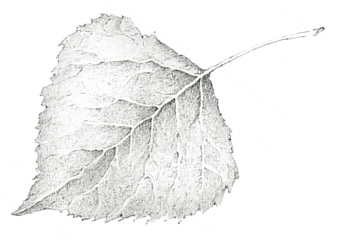
\includegraphics[width=0.6in,keepaspectratio,angle=-60]{birch_by_Aj_Vimalo_3_CMYK.png}}}

\clearpage

\section{Wild Chickens}

I'll give you a simple example. It's like wild chickens. We all know what wild chickens are like. There's no animal in the world more wary of human beings. When I first came to this forest, I taught the wild chickens. I observed them and learned many lessons from them.

At first only one of them would come past me while I was doing walking meditation. When it came close, I didn't look in its direction. Whatever it did, I didn't look in its direction. I didn't make any movement that would startle it. After a while I tried stopping still and looking at it. As soon as my eyes hit it, it ran right off. When I stopped looking at it, it would start scratching in the dirt, looking for food as before. But every time I looked at it, it would run right away.

After a little while it probably came to notice how quiet I was, so it let down its guard. But as soon as I tossed some rice in its direction, it ran right off. But I didn't care. I just kept tossing some rice out for it. After a while it would come back, but it didn't dare eat the rice. It didn't know what it was. It thought I was planning to kill it and curry it. But I didn't care whether it ate or not.

After a while it started scratching around in the dirt right there. It probably began to get a sense of what the rice was. The next day it came back to the same place and got to eat rice again. When the rice was gone, I tossed out some more for it. It ran off again. But when I kept doing this again and again, it got so that it would walk off only a little way and then come right back and eat the rice. That's when it understood.

At first the chicken saw the rice as an enemy because it wasn't acquainted with it. It didn't see it clearly. That's why it kept running off. But as it grew more tame, it came back to see what the rice actually was. That's when it knew, `This is rice. This isn't an enemy. It's not dangerous.' That's how the wild chickens here came to eat rice from that day up to the present.

In this way I learned a lesson from the wild chickens. We're just like them. Sights, sounds, smells, tastes, tactile sensations, and ideas are means for giving us knowledge of the Dhamma. They give lessons to anyone who practices. If we see them clearly in line with the truth, we'll see that that's how they are. If we don't see them clearly, they'll always be our enemies, and we'll keep running away from them all the time.

\clearpage

\section{Monkeys}

Let me give you an example. Suppose you have a pet monkey at home. It doesn't sit still. It likes to jump around and grab hold of this and that -- all kinds of things. That's how monkeys are. Now you come to the monastery. We have a monkey here too, and this monkey doesn't stay still either. It jumps around and grabs things just the same, but it doesn't irritate you, does it? Why? Because you've had a monkey. You know what monkeys are like. `The one at my home is just like your monkey here at the monastery. Your monkey is just like my monkey. They're the same monkey.' If you know just one monkey, no matter how many provinces you go to, no matter how many monkeys you see, they don't irritate you, right? That's someone who understands monkeys.

If we understand monkeys then we won't become monkeys. If you don't understand monkeys, then as soon as you see a monkey, you become a monkey yourself, right? When you see it grabbing this and that, you think, `Grrr!' You get angry and irritated. `That damned monkey!' That's someone who doesn't understand monkeys. 

Someone who understands monkeys sees that the monkey at home and the monkey at Wat Tham Saeng Phet are the same monkey, so why should they irritate you? When you see that that's what monkeys are like, that's enough. You can be at peace. If the monkey runs around, it's only the monkey running. You don't become a monkey too. You're at peace. If it jumps in front of you and behind you, you don't get irritated by the monkey. Why? Because you understand monkeys, and so you don't become a monkey. If you don't understand monkeys, you get irritated. When you get irritated, you become a monkey -- understand? This is how things grow calm.

When we know sense objects, observe sense objects: some are likable, some are not, but so what? That's their business. That's what they're like. Just like monkeys. All monkeys are the same monkey. We understand sense objects. Sometimes they're likable, sometimes they're not. That's what they're like. We have to get acquainted with them. When we're acquainted with them, we let them go. Sense objects aren't for sure. They're all inconstant, stressful, and not-self. We keep looking at them in that way. When the eye, ear, nose, tongue, body, and mind receive objects coming in, we know them, just like seeing monkeys. This monkey is just like the monkey at home. Then we can be at peace. 

\clearpage

\section{The Tree Pulls Itself Down}

Craving and desire lead us to suffering. But if we contemplate, our contemplation leans out from craving. It contemplates craving, and it pulls on the craving, shakes it up, so that it goes away or lessens on its own.

It's like a tree. Does anyone tell it what to do? Does anyone give it hints? You can't tell it what to do. You can't make it do anything. But it leans over and pulls itself down. When you look at things in this way, that's Dhamma.

\section{Heavy Lifting}

Mindfulness and alertness are like two people lifting a heavy log. A third person is watching and when he sees that the log is heavy, he comes to help. When it's heavy like that, he can't \textit{not} help. He has to help. The person helping here is discernment. It can't stay still. When there's mindfulness and alertness, discernment has to run in and join them.

\clearpage

\section{Bottled Water, Spring Water}

It's like putting water in a bottle and giving it to someone to drink. Once he's finished drinking it, he'll have to come back and ask for more -- for the water isn't water in a spring. It's water in a bottle. But if you show the spring to the person and tell him to get water there, he can sit there and keep on drinking water and won't ask you for any more, for the water never runs out.

It's the same when we see inconstancy, stress, and not-self. It goes deep, for we really know, we know all the way in. Ordinary knowledge doesn't know all the way in. If we know all the way in, it never grows stale. Whatever arises, we know it correctly -- and things disband. We know correctly without stop.

\section{Still, Flowing Water}

\enlargethispage{2\baselineskip}
Have you ever seen flowing water? Have you ever seen still water? If your mind is peaceful, it's like still, flowing water. Have you ever seen still, flowing water? There! You've only seen flowing water and still water. You've never seen still, flowing water. Right there, right where your thinking can't take you: where the mind is still but can develop discernment. When you look at your mind, it'll be like flowing water, and yet still. It looks like it's still, it looks like it's flowing, so it's called still, flowing water. That's what it's like. That's where discernment can arise.

\clearpage

\section{The Log in the Canal}

It's like cutting a log, throwing it into a canal, and letting it flow along with the water in the canal. If it doesn't get worm-eaten, doesn't rot, doesn't get smashed, doesn't get snagged on this bank or that bank, it'll keep flowing down the canal. I'm convinced that it'll ultimately reach the ocean. 

It's the same with us. If we practice in line with the Lord Buddha's way, if we follow the path he taught, if we correctly follow the current, we have to avoid two things. Which two? The two extremes that the Buddha said contemplatives shouldn't get seriously involved with. The first is sensual indulgence. The second is self-torment. These are the two banks of the canal, of the river. The log flowing down the river, following the current of the water, is our mind.

\vspace*{-\baselineskip}
\section{Waves Coming Ashore}

\enlargethispage{2\baselineskip}
Suffering and mental stress aren't for sure. They're inconstant. Keep this point in mind. When these things arise, we know them right now and we let them go. This strength of mind will gradually see more and more. When it's grown more resilient, it can suppress defilements extremely fast. As time passes, whatever arises right here disbands right here, like waves on the sea coming ashore. As soon as they reach the shore they simply dissolve. A new wave comes and it dissolves too. It can't go beyond the shore. Inconstancy, stress, and not-self are the shore of the sea. As for the sense objects that come passing in, that's all there is to them.

\clearpage

\section{The Saw}

\ldots{} But when the mind sees and knows everything, it doesn't carry the Dhamma along with it. Like this saw: they're going to use it to cut wood. When all the wood is cut and everything is done, they put the saw away. They don't need to use it anymore. The saw is the Dhamma. We have to use the Dhamma to practice the paths leading to the fruitions. When the job is done, we put the Dhamma that's there away. Like a saw used to cut wood: they cut this piece, cut that piece. When they're finished cutting, they put the saw away here. When that's the case, the saw has to be the saw; the wood has to be the wood. 

This is called reaching the point of stopping, the point that's really important. That's the end of cutting wood. We don't have to cut wood, for we've cut enough. We take the saw and put it away.
